\documentclass[1p]{elsarticle_modified}
%\bibliographystyle{elsarticle-num}

%\usepackage[colorlinks]{hyperref}
%\usepackage{abbrmath_seonhwa} %\Abb, \Ascr, \Acal ,\Abf, \Afrak
\usepackage{amsfonts}
\usepackage{amssymb}
\usepackage{amsmath}
\usepackage{amsthm}
\usepackage{scalefnt}
\usepackage{amsbsy}
\usepackage{kotex}
\usepackage{caption}
\usepackage{subfig}
\usepackage{color}
\usepackage{graphicx}
\usepackage{xcolor} %% white, black, red, green, blue, cyan, magenta, yellow
\usepackage{float}
\usepackage{setspace}
\usepackage{hyperref}

\usepackage{tikz}
\usetikzlibrary{arrows}

\usepackage{multirow}
\usepackage{array} % fixed length table
\usepackage{hhline}

%%%%%%%%%%%%%%%%%%%%%
\makeatletter
\renewcommand*\env@matrix[1][\arraystretch]{%
	\edef\arraystretch{#1}%
	\hskip -\arraycolsep
	\let\@ifnextchar\new@ifnextchar
	\array{*\c@MaxMatrixCols c}}
\makeatother %https://tex.stackexchange.com/questions/14071/how-can-i-increase-the-line-spacing-in-a-matrix
%%%%%%%%%%%%%%%

\usepackage[normalem]{ulem}

\newcommand{\msout}[1]{\ifmmode\text{\sout{\ensuremath{#1}}}\else\sout{#1}\fi}
%SOURCE: \msout is \stkout macro in https://tex.stackexchange.com/questions/20609/strikeout-in-math-mode

\newcommand{\cancel}[1]{
	\ifmmode
	{\color{red}\msout{#1}}
	\else
	{\color{red}\sout{#1}}
	\fi
}

\newcommand{\add}[1]{
	{\color{blue}\uwave{#1}}
}

\newcommand{\replace}[2]{
	\ifmmode
	{\color{red}\msout{#1}}{\color{blue}\uwave{#2}}
	\else
	{\color{red}\sout{#1}}{\color{blue}\uwave{#2}}
	\fi
}

\newcommand{\Sol}{\mathcal{S}} %segment
\newcommand{\D}{D} %diagram
\newcommand{\A}{\mathcal{A}} %arc


%%%%%%%%%%%%%%%%%%%%%%%%%%%%%5 test

\def\sl{\operatorname{\textup{SL}}(2,\Cbb)}
\def\psl{\operatorname{\textup{PSL}}(2,\Cbb)}
\def\quan{\mkern 1mu \triangleright \mkern 1mu}

\theoremstyle{definition}
\newtheorem{thm}{Theorem}[section]
\newtheorem{prop}[thm]{Proposition}
\newtheorem{lem}[thm]{Lemma}
\newtheorem{ques}[thm]{Question}
\newtheorem{cor}[thm]{Corollary}
\newtheorem{defn}[thm]{Definition}
\newtheorem{exam}[thm]{Example}
\newtheorem{rmk}[thm]{Remark}
\newtheorem{alg}[thm]{Algorithm}

\newcommand{\I}{\sqrt{-1}}
\begin{document}

%\begin{frontmatter}
%
%\title{Boundary parabolic representations of knots up to 8 crossings}
%
%%% Group authors per affiliation:
%\author{Yunhi Cho} 
%\address{Department of Mathematics, University of Seoul, Seoul, Korea}
%\ead{yhcho@uos.ac.kr}
%
%
%\author{Seonhwa Kim} %\fnref{s_kim}}
%\address{Center for Geometry and Physics, Institute for Basic Science, Pohang, 37673, Korea}
%\ead{ryeona17@ibs.re.kr}
%
%\author{Hyuk Kim}
%\address{Department of Mathematical Sciences, Seoul National University, Seoul 08826, Korea}
%\ead{hyukkim@snu.ac.kr}
%
%\author{Seokbeom Yoon}
%\address{Department of Mathematical Sciences, Seoul National University, Seoul, 08826,  Korea}
%\ead{sbyoon15@snu.ac.kr}
%
%\begin{abstract}
%We find all boundary parabolic representation of knots up to 8 crossings.
%
%\end{abstract}
%\begin{keyword}
%    \MSC[2010] 57M25 
%\end{keyword}
%
%\end{frontmatter}

%\linenumbers
%\tableofcontents
%
\newcommand\colored[1]{\textcolor{white}{\rule[-0.35ex]{0.8em}{1.4ex}}\kern-0.8em\color{red} #1}%
%\newcommand\colored[1]{\textcolor{white}{ #1}\kern-2.17ex	\textcolor{white}{ #1}\kern-1.81ex	\textcolor{white}{ #1}\kern-2.15ex\color{red}#1	}

{\Large $\underline{12n_{0036}~(K12n_{0036})}$}

\setlength{\tabcolsep}{10pt}
\renewcommand{\arraystretch}{1.6}
\vspace{1cm}\begin{tabular}{m{100pt}>{\centering\arraybackslash}m{274pt}}
\multirow{5}{120pt}{
	\centering
	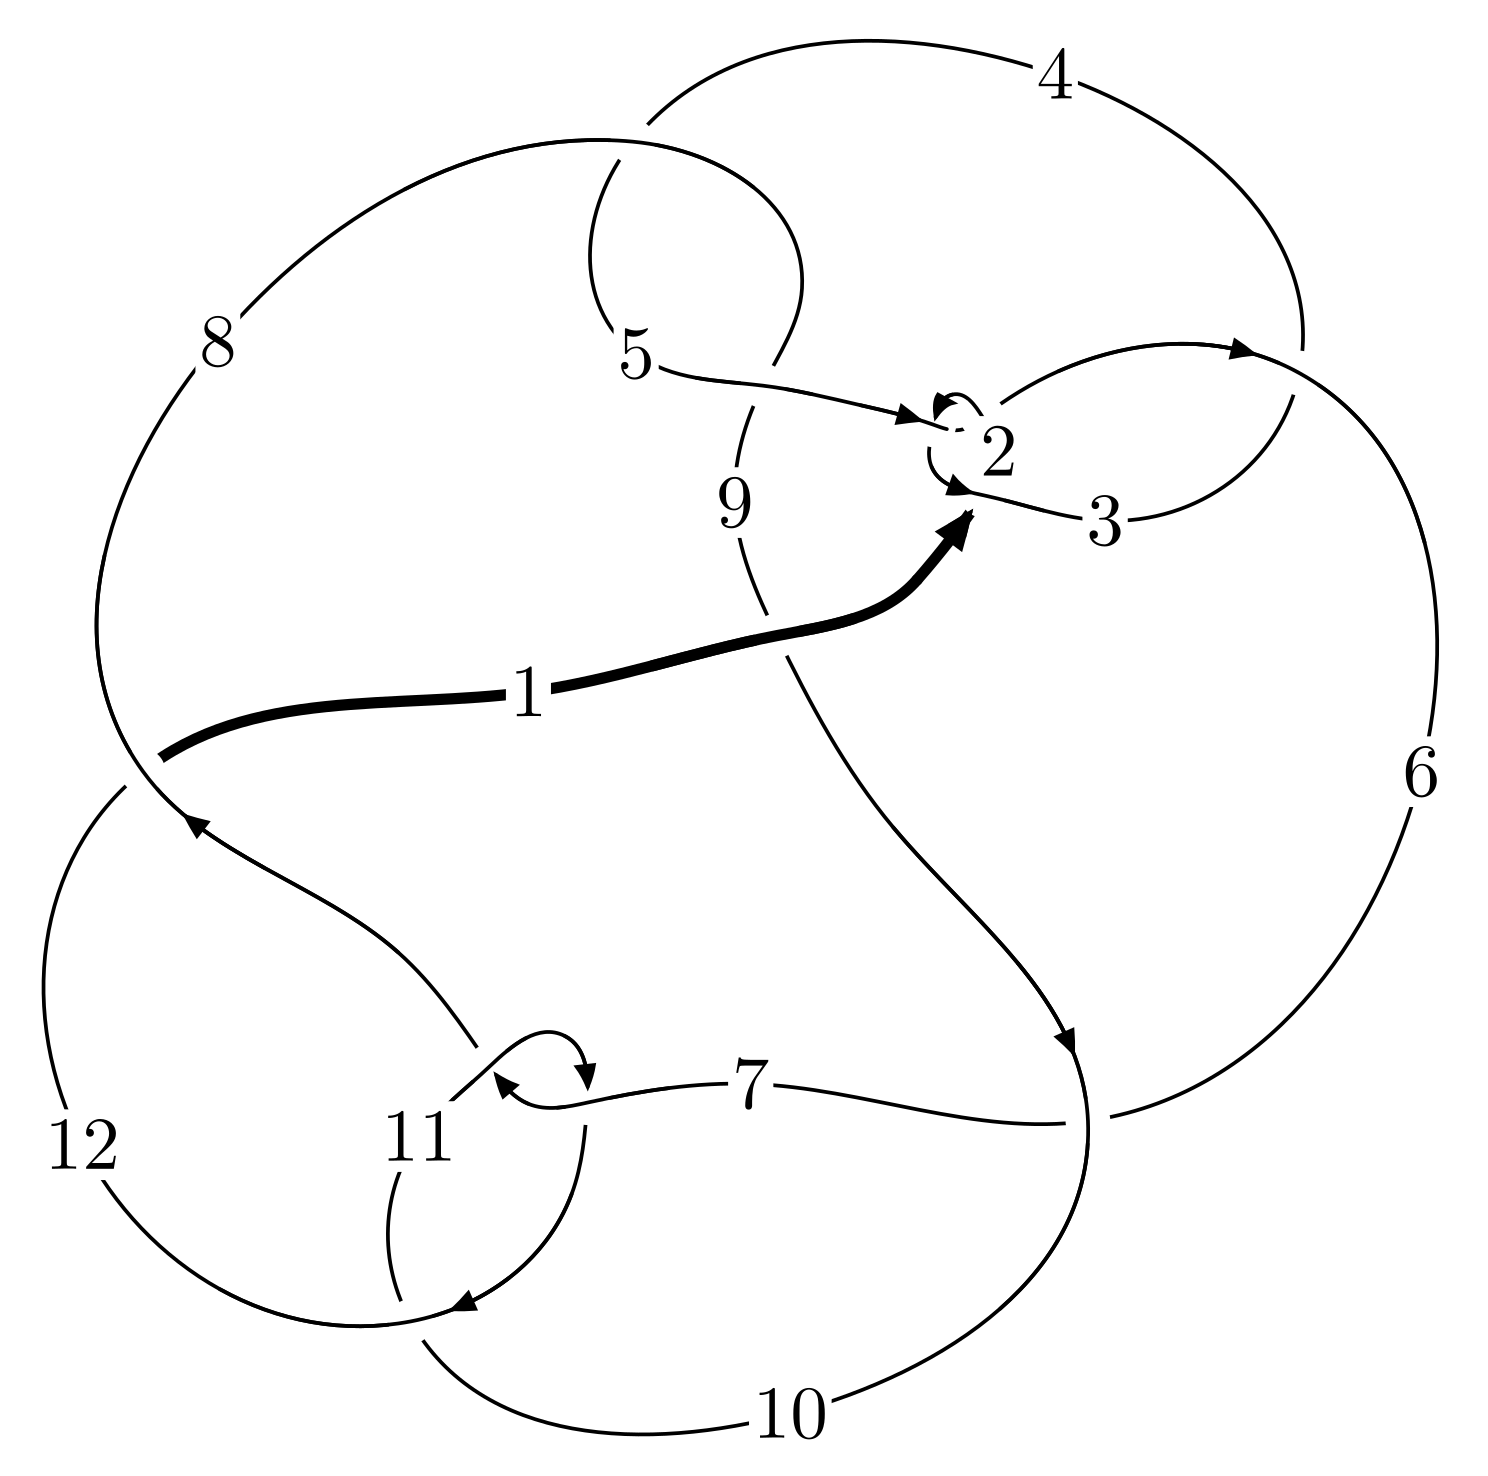
\includegraphics[width=112pt]{../../../GIT/diagram.site/Diagrams/png/2125_12n_0036.png}\\
\ \ \ A knot diagram\footnotemark}&
\allowdisplaybreaks
\textbf{Linearized knot diagam} \\
\cline{2-2}
 &
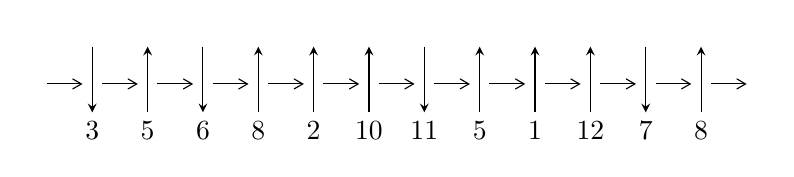
\begin{tikzpicture}[x=20pt, y=17pt]
	% nodes
	\node (C0) at (0, 0) {};
	\node (C1) at (1, 0) {};
	\node (C1U) at (1, +1) {};
	\node (C1D) at (1, -1) {3};

	\node (C2) at (2, 0) {};
	\node (C2U) at (2, +1) {};
	\node (C2D) at (2, -1) {5};

	\node (C3) at (3, 0) {};
	\node (C3U) at (3, +1) {};
	\node (C3D) at (3, -1) {6};

	\node (C4) at (4, 0) {};
	\node (C4U) at (4, +1) {};
	\node (C4D) at (4, -1) {8};

	\node (C5) at (5, 0) {};
	\node (C5U) at (5, +1) {};
	\node (C5D) at (5, -1) {2};

	\node (C6) at (6, 0) {};
	\node (C6U) at (6, +1) {};
	\node (C6D) at (6, -1) {10};

	\node (C7) at (7, 0) {};
	\node (C7U) at (7, +1) {};
	\node (C7D) at (7, -1) {11};

	\node (C8) at (8, 0) {};
	\node (C8U) at (8, +1) {};
	\node (C8D) at (8, -1) {5};

	\node (C9) at (9, 0) {};
	\node (C9U) at (9, +1) {};
	\node (C9D) at (9, -1) {1};

	\node (C10) at (10, 0) {};
	\node (C10U) at (10, +1) {};
	\node (C10D) at (10, -1) {12};

	\node (C11) at (11, 0) {};
	\node (C11U) at (11, +1) {};
	\node (C11D) at (11, -1) {7};

	\node (C12) at (12, 0) {};
	\node (C12U) at (12, +1) {};
	\node (C12D) at (12, -1) {8};
	\node (C13) at (13, 0) {};

	% arrows
	\draw[->,>={angle 60}]
	(C0) edge (C1) (C1) edge (C2) (C2) edge (C3) (C3) edge (C4) (C4) edge (C5) (C5) edge (C6) (C6) edge (C7) (C7) edge (C8) (C8) edge (C9) (C9) edge (C10) (C10) edge (C11) (C11) edge (C12) (C12) edge (C13) ;	\draw[->,>=stealth]
	(C1U) edge (C1D) (C2D) edge (C2U) (C3U) edge (C3D) (C4D) edge (C4U) (C5D) edge (C5U) (C6D) edge (C6U) (C7U) edge (C7D) (C8D) edge (C8U) (C9D) edge (C9U) (C10D) edge (C10U) (C11U) edge (C11D) (C12D) edge (C12U) ;
	\end{tikzpicture} \\
\hhline{~~} \\& 
\textbf{Solving Sequence} \\ \cline{2-2} 
 &
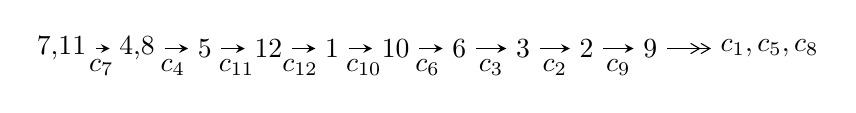
\begin{tikzpicture}[x=23pt, y=7pt]
	% node
	\node (A0) at (-1/8, 0) {7,11};
	\node (A1) at (17/16, 0) {4,8};
	\node (A2) at (17/8, 0) {5};
	\node (A3) at (25/8, 0) {12};
	\node (A4) at (33/8, 0) {1};
	\node (A5) at (41/8, 0) {10};
	\node (A6) at (49/8, 0) {6};
	\node (A7) at (57/8, 0) {3};
	\node (A8) at (65/8, 0) {2};
	\node (A9) at (73/8, 0) {9};
	\node (C1) at (1/2, -1) {$c_{7}$};
	\node (C2) at (13/8, -1) {$c_{4}$};
	\node (C3) at (21/8, -1) {$c_{11}$};
	\node (C4) at (29/8, -1) {$c_{12}$};
	\node (C5) at (37/8, -1) {$c_{10}$};
	\node (C6) at (45/8, -1) {$c_{6}$};
	\node (C7) at (53/8, -1) {$c_{3}$};
	\node (C8) at (61/8, -1) {$c_{2}$};
	\node (C9) at (69/8, -1) {$c_{9}$};
	\node (A10) at (11, 0) {$c_{1},c_{5},c_{8}$};

	% edge
	\draw[->,>=stealth]	
	(A0) edge (A1) (A1) edge (A2) (A2) edge (A3) (A3) edge (A4) (A4) edge (A5) (A5) edge (A6) (A6) edge (A7) (A7) edge (A8) (A8) edge (A9) ;
	\draw[->>,>={angle 60}]	
	(A9) edge (A10);
\end{tikzpicture} \\ 

\end{tabular} \\

\footnotetext{
The image of knot diagram is generated by the software ``\textbf{Draw programme}" developed by Andrew Bartholomew(\url{http://www.layer8.co.uk/maths/draw/index.htm\#Running-draw}), where we modified some parts for our purpose(\url{https://github.com/CATsTAILs/LinksPainter}).
}\phantom \\ \newline 
\centering \textbf{Ideals for irreducible components\footnotemark of $X_{\text{par}}$} 
 
\begin{align*}
I^u_{1}&=\langle 
4 u^{54}-8 u^{53}+\cdots+u^2+2 b,\;-4 u^{54}+8 u^{53}+\cdots+2 a+7,\;u^{55}-3 u^{54}+\cdots-3 u+1\rangle \\
I^u_{2}&=\langle 
- u^2 a+b,\;u^4- u^2 a+2 u^3+a^2- a u+3 u^2- a+2 u+1,\;u^5+u^4+2 u^3+u^2+u+1\rangle \\
\\
\end{align*}
\raggedright * 2 irreducible components of $\dim_{\mathbb{C}}=0$, with total 65 representations.\\
\footnotetext{All coefficients of polynomials are rational numbers. But the coefficients are sometimes approximated in decimal forms when there is not enough margin.}
\newpage
\renewcommand{\arraystretch}{1}
\centering \section*{I. $I^u_{1}= \langle 4 u^{54}-8 u^{53}+\cdots+u^2+2 b,\;-4 u^{54}+8 u^{53}+\cdots+2 a+7,\;u^{55}-3 u^{54}+\cdots-3 u+1 \rangle$}
\flushleft \textbf{(i) Arc colorings}\\
\begin{tabular}{m{7pt} m{180pt} m{7pt} m{180pt} }
\flushright $a_{7}=$&$\begin{pmatrix}1\\0\end{pmatrix}$ \\
\flushright $a_{11}=$&$\begin{pmatrix}0\\u\end{pmatrix}$ \\
\flushright $a_{4}=$&$\begin{pmatrix}2 u^{54}-4 u^{53}+\cdots+4 u-\frac{7}{2}\\-2 u^{54}+4 u^{53}+\cdots- u^3-\frac{1}{2} u^2\end{pmatrix}$ \\
\flushright $a_{8}=$&$\begin{pmatrix}1\\u^2\end{pmatrix}$ \\
\flushright $a_{5}=$&$\begin{pmatrix}2 u^{53}-4 u^{52}+\cdots+\frac{1}{2} u^2-\frac{3}{2}\\- u^{53}+\frac{5}{2} u^{52}+\cdots-\frac{9}{2} u^2+2 u\end{pmatrix}$ \\
\flushright $a_{12}=$&$\begin{pmatrix}- u\\u\end{pmatrix}$ \\
\flushright $a_{1}=$&$\begin{pmatrix}u^3\\u^5+u^3+u\end{pmatrix}$ \\
\flushright $a_{10}=$&$\begin{pmatrix}- u^3\\u^3+u\end{pmatrix}$ \\
\flushright $a_{6}=$&$\begin{pmatrix}- u^6- u^4+1\\u^6+2 u^4+u^2\end{pmatrix}$ \\
\flushright $a_{3}=$&$\begin{pmatrix}u^{54}-\frac{3}{2} u^{53}+\cdots+3 u-2\\- u^{54}+\frac{3}{2} u^{53}+\cdots-2 u^2+\frac{3}{2} u\end{pmatrix}$ \\
\flushright $a_{2}=$&$\begin{pmatrix}\frac{1}{2} u^{53}- u^{52}+\cdots+\frac{7}{2} u^3+1\\-\frac{1}{2} u^{53}+u^{52}+\cdots+2 u^3+\frac{1}{2} u\end{pmatrix}$ \\
\flushright $a_{9}=$&$\begin{pmatrix}- u^{11}-2 u^9-2 u^7- u^3\\- u^{13}-3 u^{11}-5 u^9-4 u^7-2 u^5+u^3+u\end{pmatrix}$\\&\end{tabular}
\flushleft \textbf{(ii) Obstruction class $= -1$}\\~\\
\flushleft \textbf{(iii) Cusp Shapes $= 4 u^{54}-\frac{33}{2} u^{53}+\cdots+20 u+\frac{1}{2}$}\\~\\
\newpage\renewcommand{\arraystretch}{1}
\flushleft \textbf{(iv) u-Polynomials at the component}\newline \\
\begin{tabular}{m{50pt}|m{274pt}}
Crossings & \hspace{64pt}u-Polynomials at each crossing \\
\hline $$\begin{aligned}c_{1}\end{aligned}$$&$\begin{aligned}
&u^{55}+32 u^{54}+\cdots-18 u-1
\end{aligned}$\\
\hline $$\begin{aligned}c_{2},c_{5}\end{aligned}$$&$\begin{aligned}
&u^{55}+6 u^{54}+\cdots-6 u-1
\end{aligned}$\\
\hline $$\begin{aligned}c_{3}\end{aligned}$$&$\begin{aligned}
&u^{55}-6 u^{54}+\cdots-18 u-1
\end{aligned}$\\
\hline $$\begin{aligned}c_{4},c_{8}\end{aligned}$$&$\begin{aligned}
&u^{55}- u^{54}+\cdots+1024 u-1024
\end{aligned}$\\
\hline $$\begin{aligned}c_{6},c_{12}\end{aligned}$$&$\begin{aligned}
&u^{55}-3 u^{54}+\cdots+379 u-73
\end{aligned}$\\
\hline $$\begin{aligned}c_{7},c_{11}\end{aligned}$$&$\begin{aligned}
&u^{55}+3 u^{54}+\cdots-3 u-1
\end{aligned}$\\
\hline $$\begin{aligned}c_{9}\end{aligned}$$&$\begin{aligned}
&u^{55}+3 u^{54}+\cdots+3 u-1
\end{aligned}$\\
\hline $$\begin{aligned}c_{10}\end{aligned}$$&$\begin{aligned}
&u^{55}-29 u^{54}+\cdots-3 u+1
\end{aligned}$\\
\hline
\end{tabular}\\~\\
\newpage\renewcommand{\arraystretch}{1}
\flushleft \textbf{(v) Riley Polynomials at the component}\newline \\
\begin{tabular}{m{50pt}|m{274pt}}
Crossings & \hspace{64pt}Riley Polynomials at each crossing \\
\hline $$\begin{aligned}c_{1}\end{aligned}$$&$\begin{aligned}
&y^{55}-12 y^{54}+\cdots-414 y-1
\end{aligned}$\\
\hline $$\begin{aligned}c_{2},c_{5}\end{aligned}$$&$\begin{aligned}
&y^{55}+32 y^{54}+\cdots-18 y-1
\end{aligned}$\\
\hline $$\begin{aligned}c_{3}\end{aligned}$$&$\begin{aligned}
&y^{55}-56 y^{54}+\cdots-2 y-1
\end{aligned}$\\
\hline $$\begin{aligned}c_{4},c_{8}\end{aligned}$$&$\begin{aligned}
&y^{55}+55 y^{54}+\cdots-15728640 y-1048576
\end{aligned}$\\
\hline $$\begin{aligned}c_{6},c_{12}\end{aligned}$$&$\begin{aligned}
&y^{55}-35 y^{54}+\cdots-79739 y-5329
\end{aligned}$\\
\hline $$\begin{aligned}c_{7},c_{11}\end{aligned}$$&$\begin{aligned}
&y^{55}+29 y^{54}+\cdots-3 y-1
\end{aligned}$\\
\hline $$\begin{aligned}c_{9}\end{aligned}$$&$\begin{aligned}
&y^{55}+65 y^{54}+\cdots-3 y-1
\end{aligned}$\\
\hline $$\begin{aligned}c_{10}\end{aligned}$$&$\begin{aligned}
&y^{55}-3 y^{54}+\cdots+29 y-1
\end{aligned}$\\
\hline
\end{tabular}\\~\\
\newpage\flushleft \textbf{(vi) Complex Volumes and Cusp Shapes}
$$\begin{array}{c|c|c}  
\text{Solutions to }I^u_{1}& \I (\text{vol} + \sqrt{-1}CS) & \text{Cusp shape}\\
 \hline 
\begin{aligned}
u &= -0.629268 + 0.778172 I \\
a &= -1.18547 + 2.27384 I \\
b &= \phantom{-}2.40744 - 0.92801 I\end{aligned}
 & -6.39910 + 2.43818 I & \phantom{-}1.82381 - 3.17764 I \\ \hline\begin{aligned}
u &= -0.629268 - 0.778172 I \\
a &= -1.18547 - 2.27384 I \\
b &= \phantom{-}2.40744 + 0.92801 I\end{aligned}
 & -6.39910 - 2.43818 I & \phantom{-}1.82381 + 3.17764 I \\ \hline\begin{aligned}
u &= -0.665364 + 0.741506 I \\
a &= \phantom{-}1.20117 - 2.12038 I \\
b &= -2.43399 + 0.82779 I\end{aligned}
 & -10.52100 - 2.56871 I & -1.299980 + 0.183319 I \\ \hline\begin{aligned}
u &= -0.665364 - 0.741506 I \\
a &= \phantom{-}1.20117 + 2.12038 I \\
b &= -2.43399 - 0.82779 I\end{aligned}
 & -10.52100 + 2.56871 I & -1.299980 - 0.183319 I \\ \hline\begin{aligned}
u &= \phantom{-}0.495253 + 0.911871 I \\
a &= \phantom{-}0.959744 - 0.326051 I \\
b &= -1.043700 + 0.351476 I\end{aligned}
 & -1.67813 - 2.05989 I & \phantom{-0.000000 -}0. + 3.35425 I \\ \hline\begin{aligned}
u &= \phantom{-}0.495253 - 0.911871 I \\
a &= \phantom{-}0.959744 + 0.326051 I \\
b &= -1.043700 - 0.351476 I\end{aligned}
 & -1.67813 + 2.05989 I & \phantom{-0.000000 } 0. - 3.35425 I \\ \hline\begin{aligned}
u &= -0.648513 + 0.820784 I \\
a &= \phantom{-}1.28463 - 2.31577 I \\
b &= -2.45034 + 0.98315 I\end{aligned}
 & -10.29050 + 7.60349 I & \phantom{-0.000000 } 0. - 6.23847 I \\ \hline\begin{aligned}
u &= -0.648513 - 0.820784 I \\
a &= \phantom{-}1.28463 + 2.31577 I \\
b &= -2.45034 - 0.98315 I\end{aligned}
 & -10.29050 - 7.60349 I & \phantom{-0.000000 -}0. + 6.23847 I \\ \hline\begin{aligned}
u &= \phantom{-}0.833853 + 0.223712 I \\
a &= \phantom{-}0.45368 - 1.70191 I \\
b &= \phantom{-}1.47926 + 0.68394 I\end{aligned}
 & -7.04904 + 9.41227 I & \phantom{-}0.67128 - 5.21491 I \\ \hline\begin{aligned}
u &= \phantom{-}0.833853 - 0.223712 I \\
a &= \phantom{-}0.45368 + 1.70191 I \\
b &= \phantom{-}1.47926 - 0.68394 I\end{aligned}
 & -7.04904 - 9.41227 I & \phantom{-}0.67128 + 5.21491 I\\
 \hline 
 \end{array}$$\newpage$$\begin{array}{c|c|c}  
\text{Solutions to }I^u_{1}& \I (\text{vol} + \sqrt{-1}CS) & \text{Cusp shape}\\
 \hline 
\begin{aligned}
u &= \phantom{-}0.256410 + 0.818450 I \\
a &= -0.479621 - 0.389548 I \\
b &= \phantom{-}0.216555 + 0.452958 I\end{aligned}
 & \phantom{-}0.489184 - 1.277770 I & \phantom{-}5.06679 + 5.28091 I \\ \hline\begin{aligned}
u &= \phantom{-}0.256410 - 0.818450 I \\
a &= -0.479621 + 0.389548 I \\
b &= \phantom{-}0.216555 - 0.452958 I\end{aligned}
 & \phantom{-}0.489184 + 1.277770 I & \phantom{-}5.06679 - 5.28091 I \\ \hline\begin{aligned}
u &= \phantom{-}0.795256 + 0.293554 I \\
a &= \phantom{-}0.39342 - 1.83875 I \\
b &= \phantom{-}1.14407 + 0.90240 I\end{aligned}
 & -8.21623 - 0.41016 I & -0.923933 + 0.833875 I \\ \hline\begin{aligned}
u &= \phantom{-}0.795256 - 0.293554 I \\
a &= \phantom{-}0.39342 + 1.83875 I \\
b &= \phantom{-}1.14407 - 0.90240 I\end{aligned}
 & -8.21623 + 0.41016 I & -0.923933 - 0.833875 I \\ \hline\begin{aligned}
u &= -0.394472 + 1.087690 I \\
a &= -1.50889 + 0.99463 I \\
b &= \phantom{-}1.397460 + 0.027206 I\end{aligned}
 & \phantom{-}1.89318 - 0.05192 I & \phantom{-0.000000 } 0 \\ \hline\begin{aligned}
u &= -0.394472 - 1.087690 I \\
a &= -1.50889 - 0.99463 I \\
b &= \phantom{-}1.397460 - 0.027206 I\end{aligned}
 & \phantom{-}1.89318 + 0.05192 I & \phantom{-0.000000 } 0 \\ \hline\begin{aligned}
u &= \phantom{-}0.795981 + 0.235146 I \\
a &= -0.47257 + 1.79828 I \\
b &= -1.27580 - 0.65059 I\end{aligned}
 & -3.68870 + 4.09212 I & \phantom{-}3.08841 - 2.21678 I \\ \hline\begin{aligned}
u &= \phantom{-}0.795981 - 0.235146 I \\
a &= -0.47257 - 1.79828 I \\
b &= -1.27580 + 0.65059 I\end{aligned}
 & -3.68870 - 4.09212 I & \phantom{-}3.08841 + 2.21678 I \\ \hline\begin{aligned}
u &= \phantom{-}0.522439 + 0.613476 I \\
a &= -0.397063 + 1.308290 I \\
b &= \phantom{-}0.133932 - 0.914279 I\end{aligned}
 & -2.54336 - 2.12347 I & -1.98097 + 3.91876 I \\ \hline\begin{aligned}
u &= \phantom{-}0.522439 - 0.613476 I \\
a &= -0.397063 - 1.308290 I \\
b &= \phantom{-}0.133932 + 0.914279 I\end{aligned}
 & -2.54336 + 2.12347 I & -1.98097 - 3.91876 I\\
 \hline 
 \end{array}$$\newpage$$\begin{array}{c|c|c}  
\text{Solutions to }I^u_{1}& \I (\text{vol} + \sqrt{-1}CS) & \text{Cusp shape}\\
 \hline 
\begin{aligned}
u &= -0.798934 + 0.043384 I \\
a &= \phantom{-}0.0979918 + 0.0882666 I \\
b &= -0.341667 - 0.572577 I\end{aligned}
 & \phantom{-}1.82991 - 1.15915 I & \phantom{-}1.11016 - 1.39618 I \\ \hline\begin{aligned}
u &= -0.798934 - 0.043384 I \\
a &= \phantom{-}0.0979918 - 0.0882666 I \\
b &= -0.341667 + 0.572577 I\end{aligned}
 & \phantom{-}1.82991 + 1.15915 I & \phantom{-}1.11016 + 1.39618 I \\ \hline\begin{aligned}
u &= \phantom{-}0.238525 + 1.182470 I \\
a &= \phantom{-}0.409365 - 0.546134 I \\
b &= -0.256958 - 0.560255 I\end{aligned}
 & -3.53580 - 3.51533 I & \phantom{-0.000000 } 0 \\ \hline\begin{aligned}
u &= \phantom{-}0.238525 - 1.182470 I \\
a &= \phantom{-}0.409365 + 0.546134 I \\
b &= -0.256958 + 0.560255 I\end{aligned}
 & -3.53580 + 3.51533 I & \phantom{-0.000000 } 0 \\ \hline\begin{aligned}
u &= \phantom{-}0.428974 + 1.129030 I \\
a &= -0.472967 - 0.859039 I \\
b &= \phantom{-}1.56190 + 1.45145 I\end{aligned}
 & \phantom{-}4.01128 - 1.20704 I & \phantom{-0.000000 } 0 \\ \hline\begin{aligned}
u &= \phantom{-}0.428974 - 1.129030 I \\
a &= -0.472967 + 0.859039 I \\
b &= \phantom{-}1.56190 - 1.45145 I\end{aligned}
 & \phantom{-}4.01128 + 1.20704 I & \phantom{-0.000000 } 0 \\ \hline\begin{aligned}
u &= \phantom{-}0.306193 + 1.184120 I \\
a &= -0.040681 + 0.327783 I \\
b &= \phantom{-}0.140846 + 0.893676 I\end{aligned}
 & \phantom{-}0.680788 + 0.637411 I & \phantom{-0.000000 } 0 \\ \hline\begin{aligned}
u &= \phantom{-}0.306193 - 1.184120 I \\
a &= -0.040681 - 0.327783 I \\
b &= \phantom{-}0.140846 - 0.893676 I\end{aligned}
 & \phantom{-}0.680788 - 0.637411 I & \phantom{-0.000000 } 0 \\ \hline\begin{aligned}
u &= \phantom{-}0.466924 + 1.132680 I \\
a &= \phantom{-}0.97235 + 1.11590 I \\
b &= -2.29775 - 1.19065 I\end{aligned}
 & \phantom{-}3.73819 - 6.60281 I & \phantom{-0.000000 } 0 \\ \hline\begin{aligned}
u &= \phantom{-}0.466924 - 1.132680 I \\
a &= \phantom{-}0.97235 - 1.11590 I \\
b &= -2.29775 + 1.19065 I\end{aligned}
 & \phantom{-}3.73819 + 6.60281 I & \phantom{-0.000000 } 0\\
 \hline 
 \end{array}$$\newpage$$\begin{array}{c|c|c}  
\text{Solutions to }I^u_{1}& \I (\text{vol} + \sqrt{-1}CS) & \text{Cusp shape}\\
 \hline 
\begin{aligned}
u &= -0.445970 + 1.141590 I \\
a &= \phantom{-}0.898688 - 0.908912 I \\
b &= -0.977538 + 0.234458 I\end{aligned}
 & \phantom{-}4.49847 + 3.98279 I & \phantom{-0.000000 } 0 \\ \hline\begin{aligned}
u &= -0.445970 - 1.141590 I \\
a &= \phantom{-}0.898688 + 0.908912 I \\
b &= -0.977538 - 0.234458 I\end{aligned}
 & \phantom{-}4.49847 - 3.98279 I & \phantom{-0.000000 } 0 \\ \hline\begin{aligned}
u &= -0.504119 + 1.119490 I \\
a &= -0.72422 + 1.48566 I \\
b &= \phantom{-}1.143880 - 0.723214 I\end{aligned}
 & \phantom{-}1.05362 + 7.50380 I & \phantom{-0.000000 } 0 \\ \hline\begin{aligned}
u &= -0.504119 - 1.119490 I \\
a &= -0.72422 - 1.48566 I \\
b &= \phantom{-}1.143880 + 0.723214 I\end{aligned}
 & \phantom{-}1.05362 - 7.50380 I & \phantom{-0.000000 } 0 \\ \hline\begin{aligned}
u &= -0.006646 + 0.753586 I \\
a &= -1.23924 - 0.91553 I \\
b &= \phantom{-}0.221110 + 1.001110 I\end{aligned}
 & \phantom{-}0.94796 - 1.37354 I & \phantom{-}8.29726 + 4.59305 I \\ \hline\begin{aligned}
u &= -0.006646 - 0.753586 I \\
a &= -1.23924 + 0.91553 I \\
b &= \phantom{-}0.221110 - 1.001110 I\end{aligned}
 & \phantom{-}0.94796 + 1.37354 I & \phantom{-}8.29726 - 4.59305 I \\ \hline\begin{aligned}
u &= \phantom{-}0.308957 + 1.222630 I \\
a &= -0.150304 - 0.576649 I \\
b &= \phantom{-}0.145017 - 0.812504 I\end{aligned}
 & -2.51298 + 5.72465 I & \phantom{-0.000000 } 0 \\ \hline\begin{aligned}
u &= \phantom{-}0.308957 - 1.222630 I \\
a &= -0.150304 + 0.576649 I \\
b &= \phantom{-}0.145017 + 0.812504 I\end{aligned}
 & -2.51298 - 5.72465 I & \phantom{-0.000000 } 0 \\ \hline\begin{aligned}
u &= \phantom{-}0.562093 + 1.144990 I \\
a &= -2.01573 - 0.76521 I \\
b &= \phantom{-}2.80550 - 0.09124 I\end{aligned}
 & -5.70109 - 4.64931 I & \phantom{-0.000000 } 0 \\ \hline\begin{aligned}
u &= \phantom{-}0.562093 - 1.144990 I \\
a &= -2.01573 + 0.76521 I \\
b &= \phantom{-}2.80550 + 0.09124 I\end{aligned}
 & -5.70109 + 4.64931 I & \phantom{-0.000000 } 0\\
 \hline 
 \end{array}$$\newpage$$\begin{array}{c|c|c}  
\text{Solutions to }I^u_{1}& \I (\text{vol} + \sqrt{-1}CS) & \text{Cusp shape}\\
 \hline 
\begin{aligned}
u &= \phantom{-}0.543221 + 1.166590 I \\
a &= \phantom{-}2.03351 + 1.01526 I \\
b &= -3.03630 - 0.03630 I\end{aligned}
 & -0.93977 - 9.06965 I & \phantom{-0.000000 } 0 \\ \hline\begin{aligned}
u &= \phantom{-}0.543221 - 1.166590 I \\
a &= \phantom{-}2.03351 - 1.01526 I \\
b &= -3.03630 + 0.03630 I\end{aligned}
 & -0.93977 + 9.06965 I & \phantom{-0.000000 } 0 \\ \hline\begin{aligned}
u &= -0.437917 + 1.210660 I \\
a &= \phantom{-}0.760392 + 0.093272 I \\
b &= -0.473659 - 0.350913 I\end{aligned}
 & \phantom{-}5.51374 + 3.19066 I & \phantom{-0.000000 } 0 \\ \hline\begin{aligned}
u &= -0.437917 - 1.210660 I \\
a &= \phantom{-}0.760392 - 0.093272 I \\
b &= -0.473659 + 0.350913 I\end{aligned}
 & \phantom{-}5.51374 - 3.19066 I & \phantom{-0.000000 } 0 \\ \hline\begin{aligned}
u &= -0.472267 + 1.211330 I \\
a &= -0.320209 - 0.705624 I \\
b &= -0.049480 + 0.606670 I\end{aligned}
 & \phantom{-}5.27082 + 5.76680 I & \phantom{-0.000000 } 0 \\ \hline\begin{aligned}
u &= -0.472267 - 1.211330 I \\
a &= -0.320209 + 0.705624 I \\
b &= -0.049480 - 0.606670 I\end{aligned}
 & \phantom{-}5.27082 - 5.76680 I & \phantom{-0.000000 } 0 \\ \hline\begin{aligned}
u &= \phantom{-}0.550577 + 1.182870 I \\
a &= -2.18265 - 1.04941 I \\
b &= \phantom{-}3.13565 - 0.09179 I\end{aligned}
 & -4.1957 - 14.5134 I & \phantom{-0.000000 } 0 \\ \hline\begin{aligned}
u &= \phantom{-}0.550577 - 1.182870 I \\
a &= -2.18265 + 1.04941 I \\
b &= \phantom{-}3.13565 + 0.09179 I\end{aligned}
 & -4.1957 + 14.5134 I & \phantom{-0.000000 } 0 \\ \hline\begin{aligned}
u &= -0.627951 + 0.254073 I \\
a &= -0.152563 + 0.574638 I \\
b &= \phantom{-}1.207510 + 0.084242 I\end{aligned}
 & -1.41318 - 3.06748 I & \phantom{-}0.44741 + 4.00287 I \\ \hline\begin{aligned}
u &= -0.627951 - 0.254073 I \\
a &= -0.152563 - 0.574638 I \\
b &= \phantom{-}1.207510 - 0.084242 I\end{aligned}
 & -1.41318 + 3.06748 I & \phantom{-}0.44741 - 4.00287 I\\
 \hline 
 \end{array}$$\newpage$$\begin{array}{c|c|c}  
\text{Solutions to }I^u_{1}& \I (\text{vol} + \sqrt{-1}CS) & \text{Cusp shape}\\
 \hline 
\begin{aligned}
u &= -0.245896 + 0.622986 I \\
a &= \phantom{-}1.09436 + 1.93010 I \\
b &= \phantom{-}0.66336 - 1.42809 I\end{aligned}
 & \phantom{-}0.12059 + 2.86553 I & \phantom{-}2.35860 + 0.38000 I \\ \hline\begin{aligned}
u &= -0.245896 - 0.622986 I \\
a &= \phantom{-}1.09436 - 1.93010 I \\
b &= \phantom{-}0.66336 + 1.42809 I\end{aligned}
 & \phantom{-}0.12059 - 2.86553 I & \phantom{-}2.35860 - 0.38000 I \\ \hline\begin{aligned}
u &= -0.626935\phantom{ +0.000000I} \\
a &= -0.0900412\phantom{ +0.000000I} \\
b &= -0.792661\phantom{ +0.000000I}\end{aligned}
 & \phantom{-}1.42624\phantom{ +0.000000I} & \phantom{-}7.14390\phantom{ +0.000000I} \\ \hline\begin{aligned}
u &= \phantom{-}0.586127 + 0.078855 I \\
a &= -0.17208 + 2.32899 I \\
b &= -0.269979 - 0.036468 I\end{aligned}
 & \phantom{-}0.91267 + 2.50494 I & \phantom{-}1.11924 - 3.76856 I \\ \hline\begin{aligned}
u &= \phantom{-}0.586127 - 0.078855 I \\
a &= -0.17208 - 2.32899 I \\
b &= -0.269979 + 0.036468 I\end{aligned}
 & \phantom{-}0.91267 - 2.50494 I & \phantom{-}1.11924 + 3.76856 I\\
 \hline 
 \end{array}$$\newpage\newpage\renewcommand{\arraystretch}{1}
\centering \section*{II. $I^u_{2}= \langle - u^2 a+b,\;u^4- u^2 a+2 u^3+a^2- a u+3 u^2- a+2 u+1,\;u^5+u^4+2 u^3+u^2+u+1 \rangle$}
\flushleft \textbf{(i) Arc colorings}\\
\begin{tabular}{m{7pt} m{180pt} m{7pt} m{180pt} }
\flushright $a_{7}=$&$\begin{pmatrix}1\\0\end{pmatrix}$ \\
\flushright $a_{11}=$&$\begin{pmatrix}0\\u\end{pmatrix}$ \\
\flushright $a_{4}=$&$\begin{pmatrix}a\\u^2 a\end{pmatrix}$ \\
\flushright $a_{8}=$&$\begin{pmatrix}1\\u^2\end{pmatrix}$ \\
\flushright $a_{5}=$&$\begin{pmatrix}a\\u^2 a\end{pmatrix}$ \\
\flushright $a_{12}=$&$\begin{pmatrix}- u\\u\end{pmatrix}$ \\
\flushright $a_{1}=$&$\begin{pmatrix}u^3\\- u^4- u^3- u^2-1\end{pmatrix}$ \\
\flushright $a_{10}=$&$\begin{pmatrix}- u^3\\u^3+u\end{pmatrix}$ \\
\flushright $a_{6}=$&$\begin{pmatrix}- u^3\\u^4+u^3+u^2+1\end{pmatrix}$ \\
\flushright $a_{3}=$&$\begin{pmatrix}- u^3 a\\u^3 a+a u\end{pmatrix}$ \\
\flushright $a_{2}=$&$\begin{pmatrix}- u^3 a- u^2- u-1\\u^3 a- u^4- u^3+a u- u^2\end{pmatrix}$ \\
\flushright $a_{9}=$&$\begin{pmatrix}1\\u^2\end{pmatrix}$\\&\end{tabular}
\flushleft \textbf{(ii) Obstruction class $= 1$}\\~\\
\flushleft \textbf{(iii) Cusp Shapes $= -5 u^3 a+u^4+6 u^3-6 a u+7 u^2- a+6 u+7$}\\~\\
\newpage\renewcommand{\arraystretch}{1}
\flushleft \textbf{(iv) u-Polynomials at the component}\newline \\
\begin{tabular}{m{50pt}|m{274pt}}
Crossings & \hspace{64pt}u-Polynomials at each crossing \\
\hline $$\begin{aligned}c_{1},c_{3},c_{5}\end{aligned}$$&$\begin{aligned}
&(u^2- u+1)^5
\end{aligned}$\\
\hline $$\begin{aligned}c_{2}\end{aligned}$$&$\begin{aligned}
&(u^2+u+1)^5
\end{aligned}$\\
\hline $$\begin{aligned}c_{4},c_{8}\end{aligned}$$&$\begin{aligned}
&u^{10}
\end{aligned}$\\
\hline $$\begin{aligned}c_{6},c_{9}\end{aligned}$$&$\begin{aligned}
&(u^5- u^4-2 u^3+u^2+u+1)^2
\end{aligned}$\\
\hline $$\begin{aligned}c_{7}\end{aligned}$$&$\begin{aligned}
&(u^5+u^4+2 u^3+u^2+u+1)^2
\end{aligned}$\\
\hline $$\begin{aligned}c_{10}\end{aligned}$$&$\begin{aligned}
&(u^5+3 u^4+4 u^3+u^2- u-1)^2
\end{aligned}$\\
\hline $$\begin{aligned}c_{11}\end{aligned}$$&$\begin{aligned}
&(u^5- u^4+2 u^3- u^2+u-1)^2
\end{aligned}$\\
\hline $$\begin{aligned}c_{12}\end{aligned}$$&$\begin{aligned}
&(u^5+u^4-2 u^3- u^2+u-1)^2
\end{aligned}$\\
\hline
\end{tabular}\\~\\
\newpage\renewcommand{\arraystretch}{1}
\flushleft \textbf{(v) Riley Polynomials at the component}\newline \\
\begin{tabular}{m{50pt}|m{274pt}}
Crossings & \hspace{64pt}Riley Polynomials at each crossing \\
\hline $$\begin{aligned}c_{1},c_{2},c_{3}\\c_{5}\end{aligned}$$&$\begin{aligned}
&(y^2+y+1)^5
\end{aligned}$\\
\hline $$\begin{aligned}c_{4},c_{8}\end{aligned}$$&$\begin{aligned}
&y^{10}
\end{aligned}$\\
\hline $$\begin{aligned}c_{6},c_{9},c_{12}\end{aligned}$$&$\begin{aligned}
&(y^5-5 y^4+8 y^3-3 y^2- y-1)^2
\end{aligned}$\\
\hline $$\begin{aligned}c_{7},c_{11}\end{aligned}$$&$\begin{aligned}
&(y^5+3 y^4+4 y^3+y^2- y-1)^2
\end{aligned}$\\
\hline $$\begin{aligned}c_{10}\end{aligned}$$&$\begin{aligned}
&(y^5- y^4+8 y^3-3 y^2+3 y-1)^2
\end{aligned}$\\
\hline
\end{tabular}\\~\\
\newpage\flushleft \textbf{(vi) Complex Volumes and Cusp Shapes}
$$\begin{array}{c|c|c}  
\text{Solutions to }I^u_{2}& \I (\text{vol} + \sqrt{-1}CS) & \text{Cusp shape}\\
 \hline 
\begin{aligned}
u &= \phantom{-}0.339110 + 0.822375 I \\
a &= -0.80632 + 1.36366 I \\
b &= -0.307991 - 1.215160 I\end{aligned}
 & \phantom{-}0.32910 - 3.56046 I & \phantom{-}5.91654 + 9.74472 I \\ \hline\begin{aligned}
u &= \phantom{-}0.339110 + 0.822375 I \\
a &= \phantom{-}1.58413 + 0.01647 I \\
b &= -0.898363 + 0.874307 I\end{aligned}
 & \phantom{-}0.329100 + 0.499304 I & \phantom{-}1.60756 + 0.92266 I \\ \hline\begin{aligned}
u &= \phantom{-}0.339110 - 0.822375 I \\
a &= -0.80632 - 1.36366 I \\
b &= -0.307991 + 1.215160 I\end{aligned}
 & \phantom{-}0.32910 + 3.56046 I & \phantom{-}5.91654 - 9.74472 I \\ \hline\begin{aligned}
u &= \phantom{-}0.339110 - 0.822375 I \\
a &= \phantom{-}1.58413 - 0.01647 I \\
b &= -0.898363 - 0.874307 I\end{aligned}
 & \phantom{-}0.329100 - 0.499304 I & \phantom{-}1.60756 - 0.92266 I \\ \hline\begin{aligned}
u &= -0.766826\phantom{ +0.000000I} \\
a &= \phantom{-}0.410598 + 0.711177 I \\
b &= \phantom{-}0.241441 + 0.418187 I\end{aligned}
 & \phantom{-}2.40108 - 2.02988 I & \phantom{-}6.55976 + 4.16430 I \\ \hline\begin{aligned}
u &= -0.766826\phantom{ +0.000000I} \\
a &= \phantom{-}0.410598 - 0.711177 I \\
b &= \phantom{-}0.241441 - 0.418187 I\end{aligned}
 & \phantom{-}2.40108 + 2.02988 I & \phantom{-}6.55976 - 4.16430 I \\ \hline\begin{aligned}
u &= -0.455697 + 1.200150 I \\
a &= -0.252108 + 0.649344 I \\
b &= \phantom{-}1.021040 - 0.524691 I\end{aligned}
 & \phantom{-}5.87256 + 6.43072 I & \phantom{-}10.62344 - 8.02599 I \\ \hline\begin{aligned}
u &= -0.455697 + 1.200150 I \\
a &= -0.436295 - 0.543004 I \\
b &= -0.056121 + 1.146590 I\end{aligned}
 & \phantom{-}5.87256 + 2.37095 I & \phantom{-}9.29269 + 1.50431 I \\ \hline\begin{aligned}
u &= -0.455697 - 1.200150 I \\
a &= -0.252108 - 0.649344 I \\
b &= \phantom{-}1.021040 + 0.524691 I\end{aligned}
 & \phantom{-}5.87256 - 6.43072 I & \phantom{-}10.62344 + 8.02599 I \\ \hline\begin{aligned}
u &= -0.455697 - 1.200150 I \\
a &= -0.436295 + 0.543004 I \\
b &= -0.056121 - 1.146590 I\end{aligned}
 & \phantom{-}5.87256 - 2.37095 I & \phantom{-}9.29269 - 1.50431 I\\
 \hline 
 \end{array}$$\newpage
\newpage\renewcommand{\arraystretch}{1}
\centering \section*{ III. u-Polynomials}
\begin{tabular}{m{50pt}|m{274pt}}
Crossings & \hspace{64pt}u-Polynomials at each crossing \\
\hline $$\begin{aligned}c_{1}\end{aligned}$$&$\begin{aligned}
&((u^2- u+1)^5)(u^{55}+32 u^{54}+\cdots-18 u-1)
\end{aligned}$\\
\hline $$\begin{aligned}c_{2}\end{aligned}$$&$\begin{aligned}
&((u^2+u+1)^5)(u^{55}+6 u^{54}+\cdots-6 u-1)
\end{aligned}$\\
\hline $$\begin{aligned}c_{3}\end{aligned}$$&$\begin{aligned}
&((u^2- u+1)^5)(u^{55}-6 u^{54}+\cdots-18 u-1)
\end{aligned}$\\
\hline $$\begin{aligned}c_{4},c_{8}\end{aligned}$$&$\begin{aligned}
&u^{10}(u^{55}- u^{54}+\cdots+1024 u-1024)
\end{aligned}$\\
\hline $$\begin{aligned}c_{5}\end{aligned}$$&$\begin{aligned}
&((u^2- u+1)^5)(u^{55}+6 u^{54}+\cdots-6 u-1)
\end{aligned}$\\
\hline $$\begin{aligned}c_{6}\end{aligned}$$&$\begin{aligned}
&((u^5- u^4-2 u^3+u^2+u+1)^2)(u^{55}-3 u^{54}+\cdots+379 u-73)
\end{aligned}$\\
\hline $$\begin{aligned}c_{7}\end{aligned}$$&$\begin{aligned}
&((u^5+u^4+2 u^3+u^2+u+1)^2)(u^{55}+3 u^{54}+\cdots-3 u-1)
\end{aligned}$\\
\hline $$\begin{aligned}c_{9}\end{aligned}$$&$\begin{aligned}
&((u^5- u^4-2 u^3+u^2+u+1)^2)(u^{55}+3 u^{54}+\cdots+3 u-1)
\end{aligned}$\\
\hline $$\begin{aligned}c_{10}\end{aligned}$$&$\begin{aligned}
&((u^5+3 u^4+4 u^3+u^2- u-1)^2)(u^{55}-29 u^{54}+\cdots-3 u+1)
\end{aligned}$\\
\hline $$\begin{aligned}c_{11}\end{aligned}$$&$\begin{aligned}
&((u^5- u^4+2 u^3- u^2+u-1)^2)(u^{55}+3 u^{54}+\cdots-3 u-1)
\end{aligned}$\\
\hline $$\begin{aligned}c_{12}\end{aligned}$$&$\begin{aligned}
&((u^5+u^4-2 u^3- u^2+u-1)^2)(u^{55}-3 u^{54}+\cdots+379 u-73)
\end{aligned}$\\
\hline
\end{tabular}\newpage\renewcommand{\arraystretch}{1}
\centering \section*{ IV. Riley Polynomials}
\begin{tabular}{m{50pt}|m{274pt}}
Crossings & \hspace{64pt}Riley Polynomials at each crossing \\
\hline $$\begin{aligned}c_{1}\end{aligned}$$&$\begin{aligned}
&((y^2+y+1)^5)(y^{55}-12 y^{54}+\cdots-414 y-1)
\end{aligned}$\\
\hline $$\begin{aligned}c_{2},c_{5}\end{aligned}$$&$\begin{aligned}
&((y^2+y+1)^5)(y^{55}+32 y^{54}+\cdots-18 y-1)
\end{aligned}$\\
\hline $$\begin{aligned}c_{3}\end{aligned}$$&$\begin{aligned}
&((y^2+y+1)^5)(y^{55}-56 y^{54}+\cdots-2 y-1)
\end{aligned}$\\
\hline $$\begin{aligned}c_{4},c_{8}\end{aligned}$$&$\begin{aligned}
&y^{10}(y^{55}+55 y^{54}+\cdots-1.57286\times10^{7} y-1048576)
\end{aligned}$\\
\hline $$\begin{aligned}c_{6},c_{12}\end{aligned}$$&$\begin{aligned}
&((y^5-5 y^4+8 y^3-3 y^2- y-1)^2)(y^{55}-35 y^{54}+\cdots-79739 y-5329)
\end{aligned}$\\
\hline $$\begin{aligned}c_{7},c_{11}\end{aligned}$$&$\begin{aligned}
&((y^5+3 y^4+4 y^3+y^2- y-1)^2)(y^{55}+29 y^{54}+\cdots-3 y-1)
\end{aligned}$\\
\hline $$\begin{aligned}c_{9}\end{aligned}$$&$\begin{aligned}
&((y^5-5 y^4+8 y^3-3 y^2- y-1)^2)(y^{55}+65 y^{54}+\cdots-3 y-1)
\end{aligned}$\\
\hline $$\begin{aligned}c_{10}\end{aligned}$$&$\begin{aligned}
&((y^5- y^4+8 y^3-3 y^2+3 y-1)^2)(y^{55}-3 y^{54}+\cdots+29 y-1)
\end{aligned}$\\
\hline
\end{tabular}
\vskip 2pc
\end{document}